\documentclass[a4paper]{article}

\usepackage{fullpage} % Package to use full page
\usepackage{parskip} % Package to tweak paragraph skipping
\usepackage{tikz} % Package for drawing
\usepackage{amsmath}
\usepackage{siunitx} % Package for scientific units
\usepackage{amsfonts}
\usepackage{amssymb}
\usepackage{hyperref}
\usepackage[utf8]{inputenc}
\usepackage[english]{babel}
\usepackage{multicol}
\usepackage{graphicx} % Package for including images
\usepackage{mathtools}
\usepackage{pgfplots}
\graphicspath{ {./images/} }

\newcommand\tab[1][0.5cm]{\hspace*{#1}}
\DeclarePairedDelimiter\Floor\lfloor\rfloor
\DeclarePairedDelimiter\Ceil\lceil\rceil
\usepgfplotslibrary{polar}
\usepgflibrary{shapes.geometric}
\usetikzlibrary{calc}
\pgfplotsset{my style/.append style={axis x line=middle, axis y line=
middle, xlabel={$x$}, ylabel={$y$} }}
\pgfplotsset{compat=1.14}
\usepgfplotslibrary{fillbetween}


\title{LHW 1}
\author{Adrian Darian}
\date{2/1/2021}

\begin{document}
  
\maketitle

Complete the tasks over at \url{https://dsollberger.shinyapps.io/Math32LearnR1/}

\begin{itemize}
	\item take a screenshot of each page of this assignment
	\item copy and paste the screenshots onto a Word document (or Google Doc or equivalent)
	\item save as a PDF
	\item be sure that your name appears on the document
	\item upload the PDF back to our CatCourses page
\end{itemize}

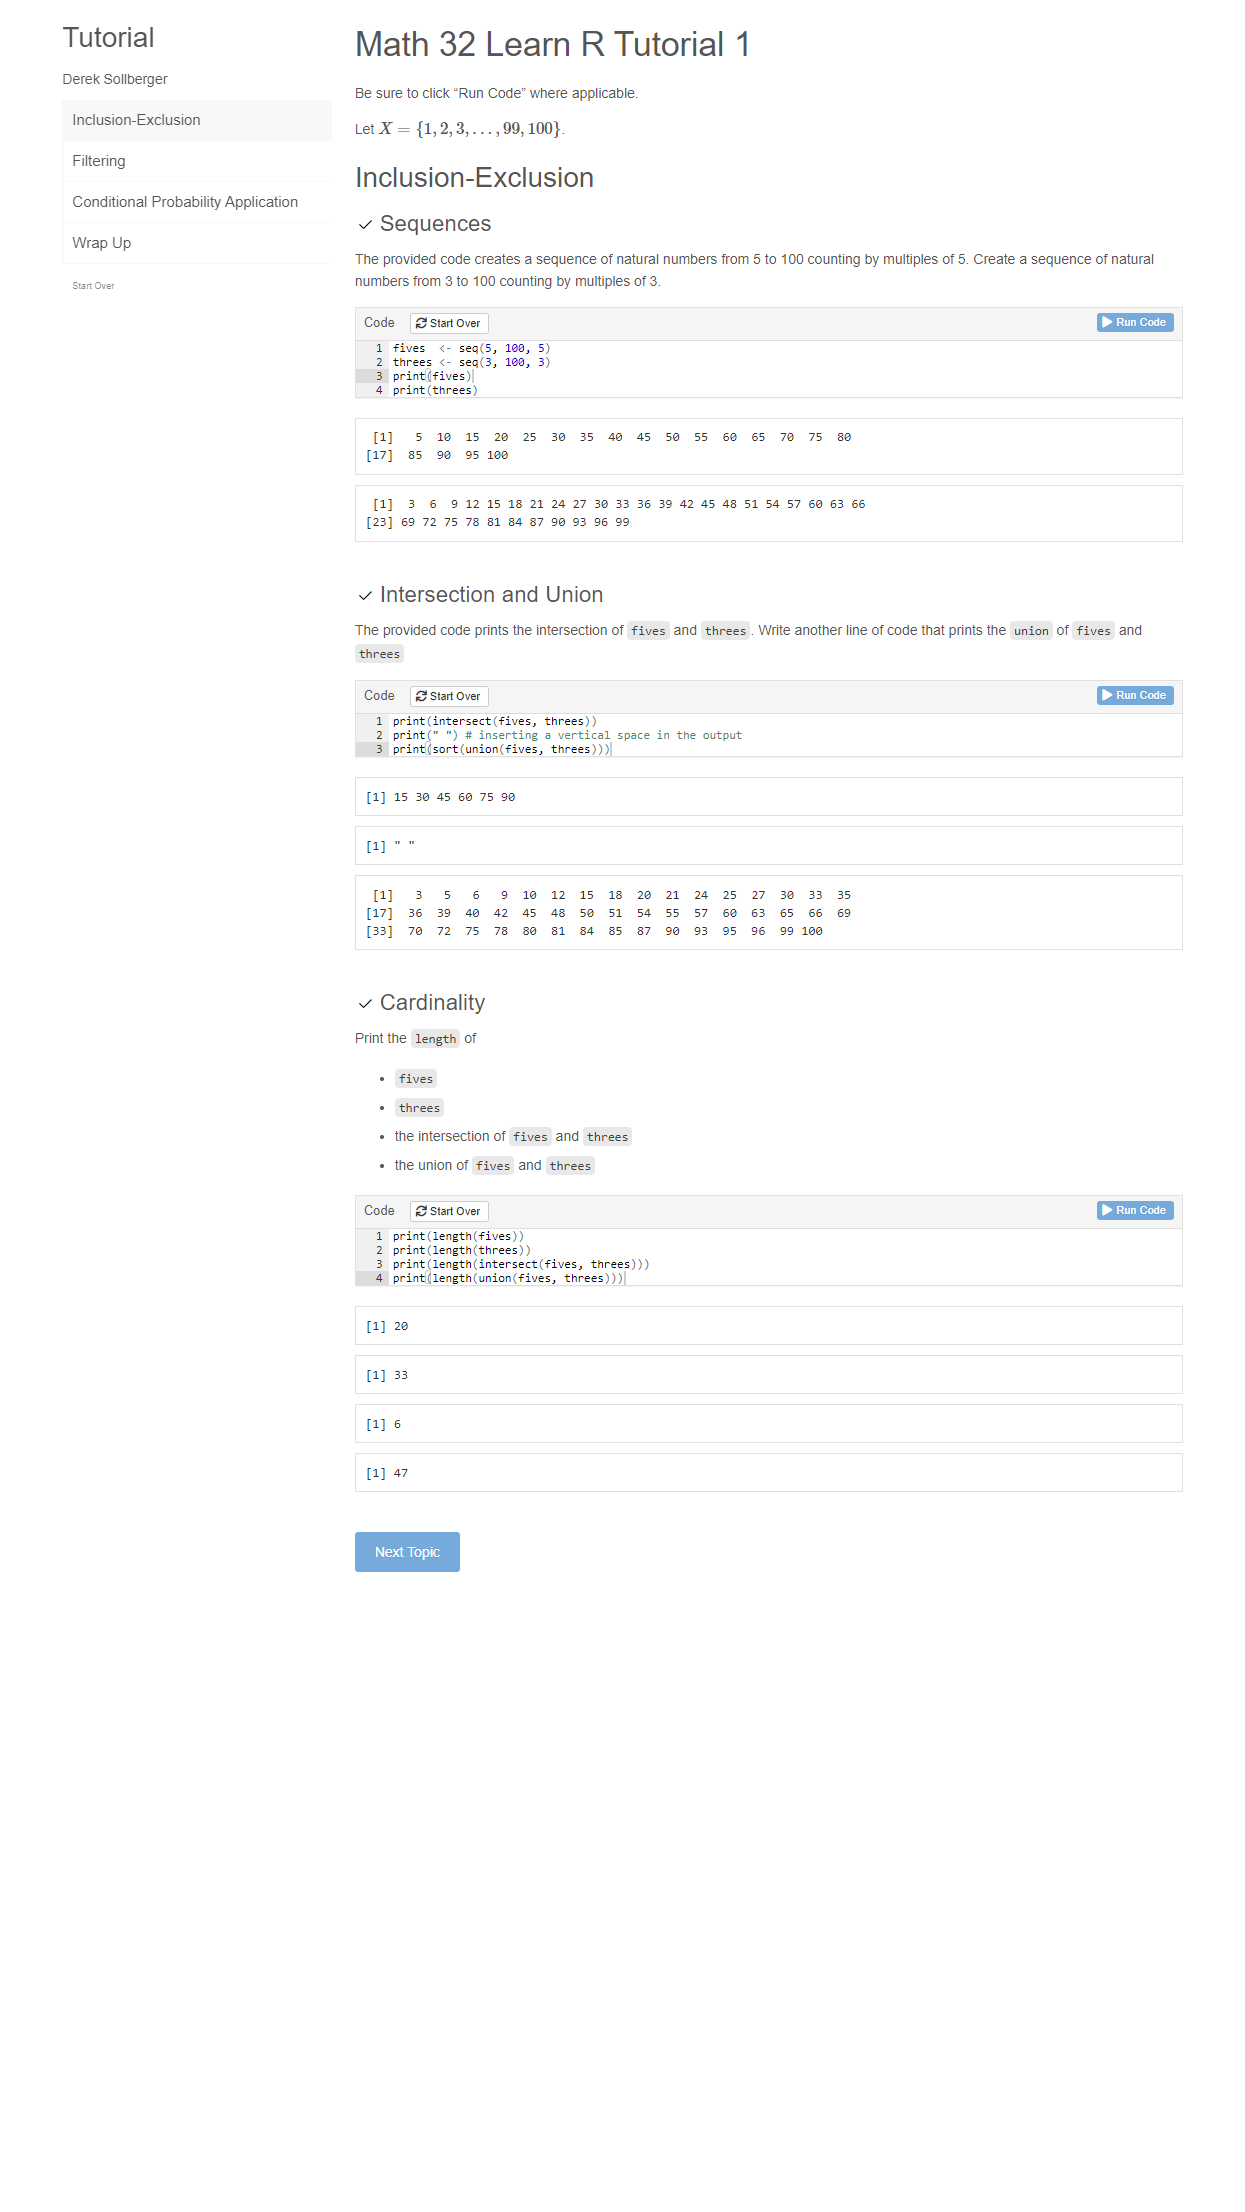
\includegraphics[scale=0.4]{page_1.png} \\
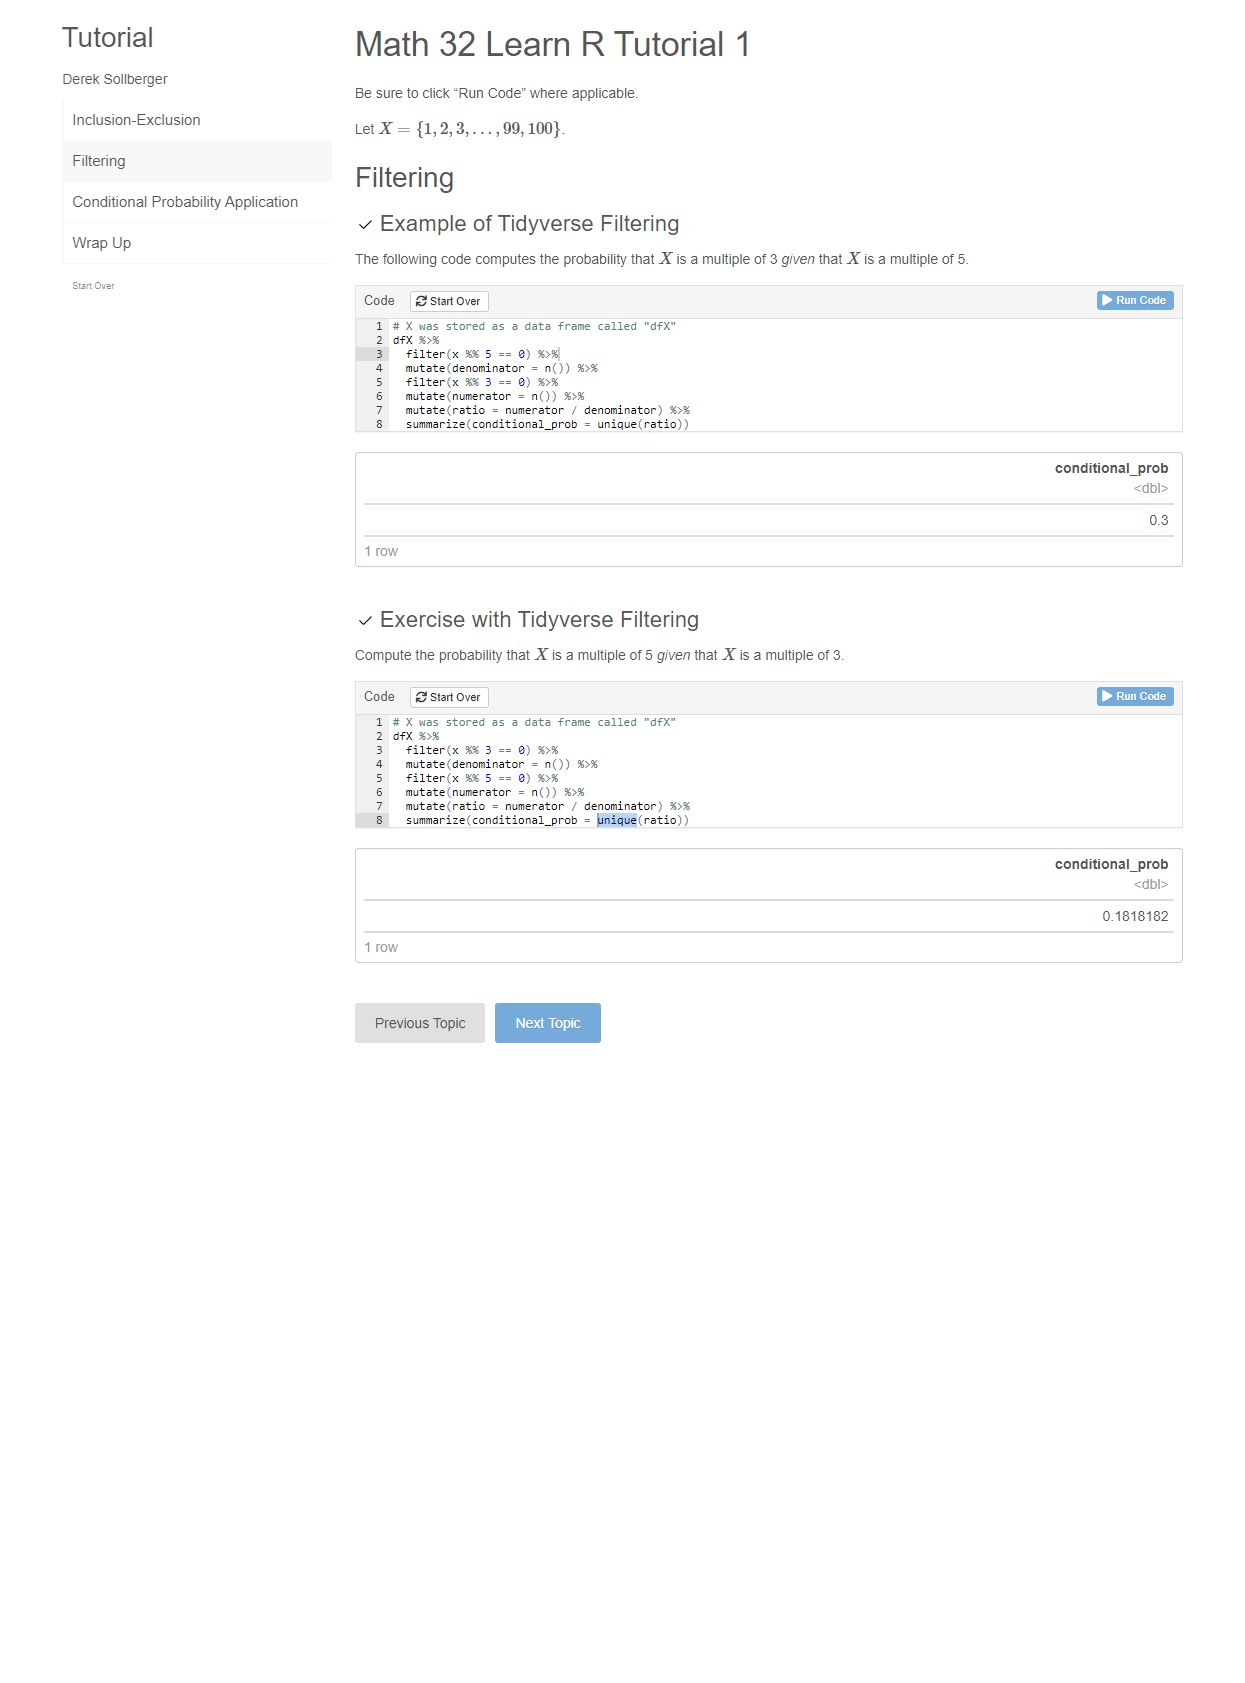
\includegraphics[scale=0.4]{page_2.png} \\
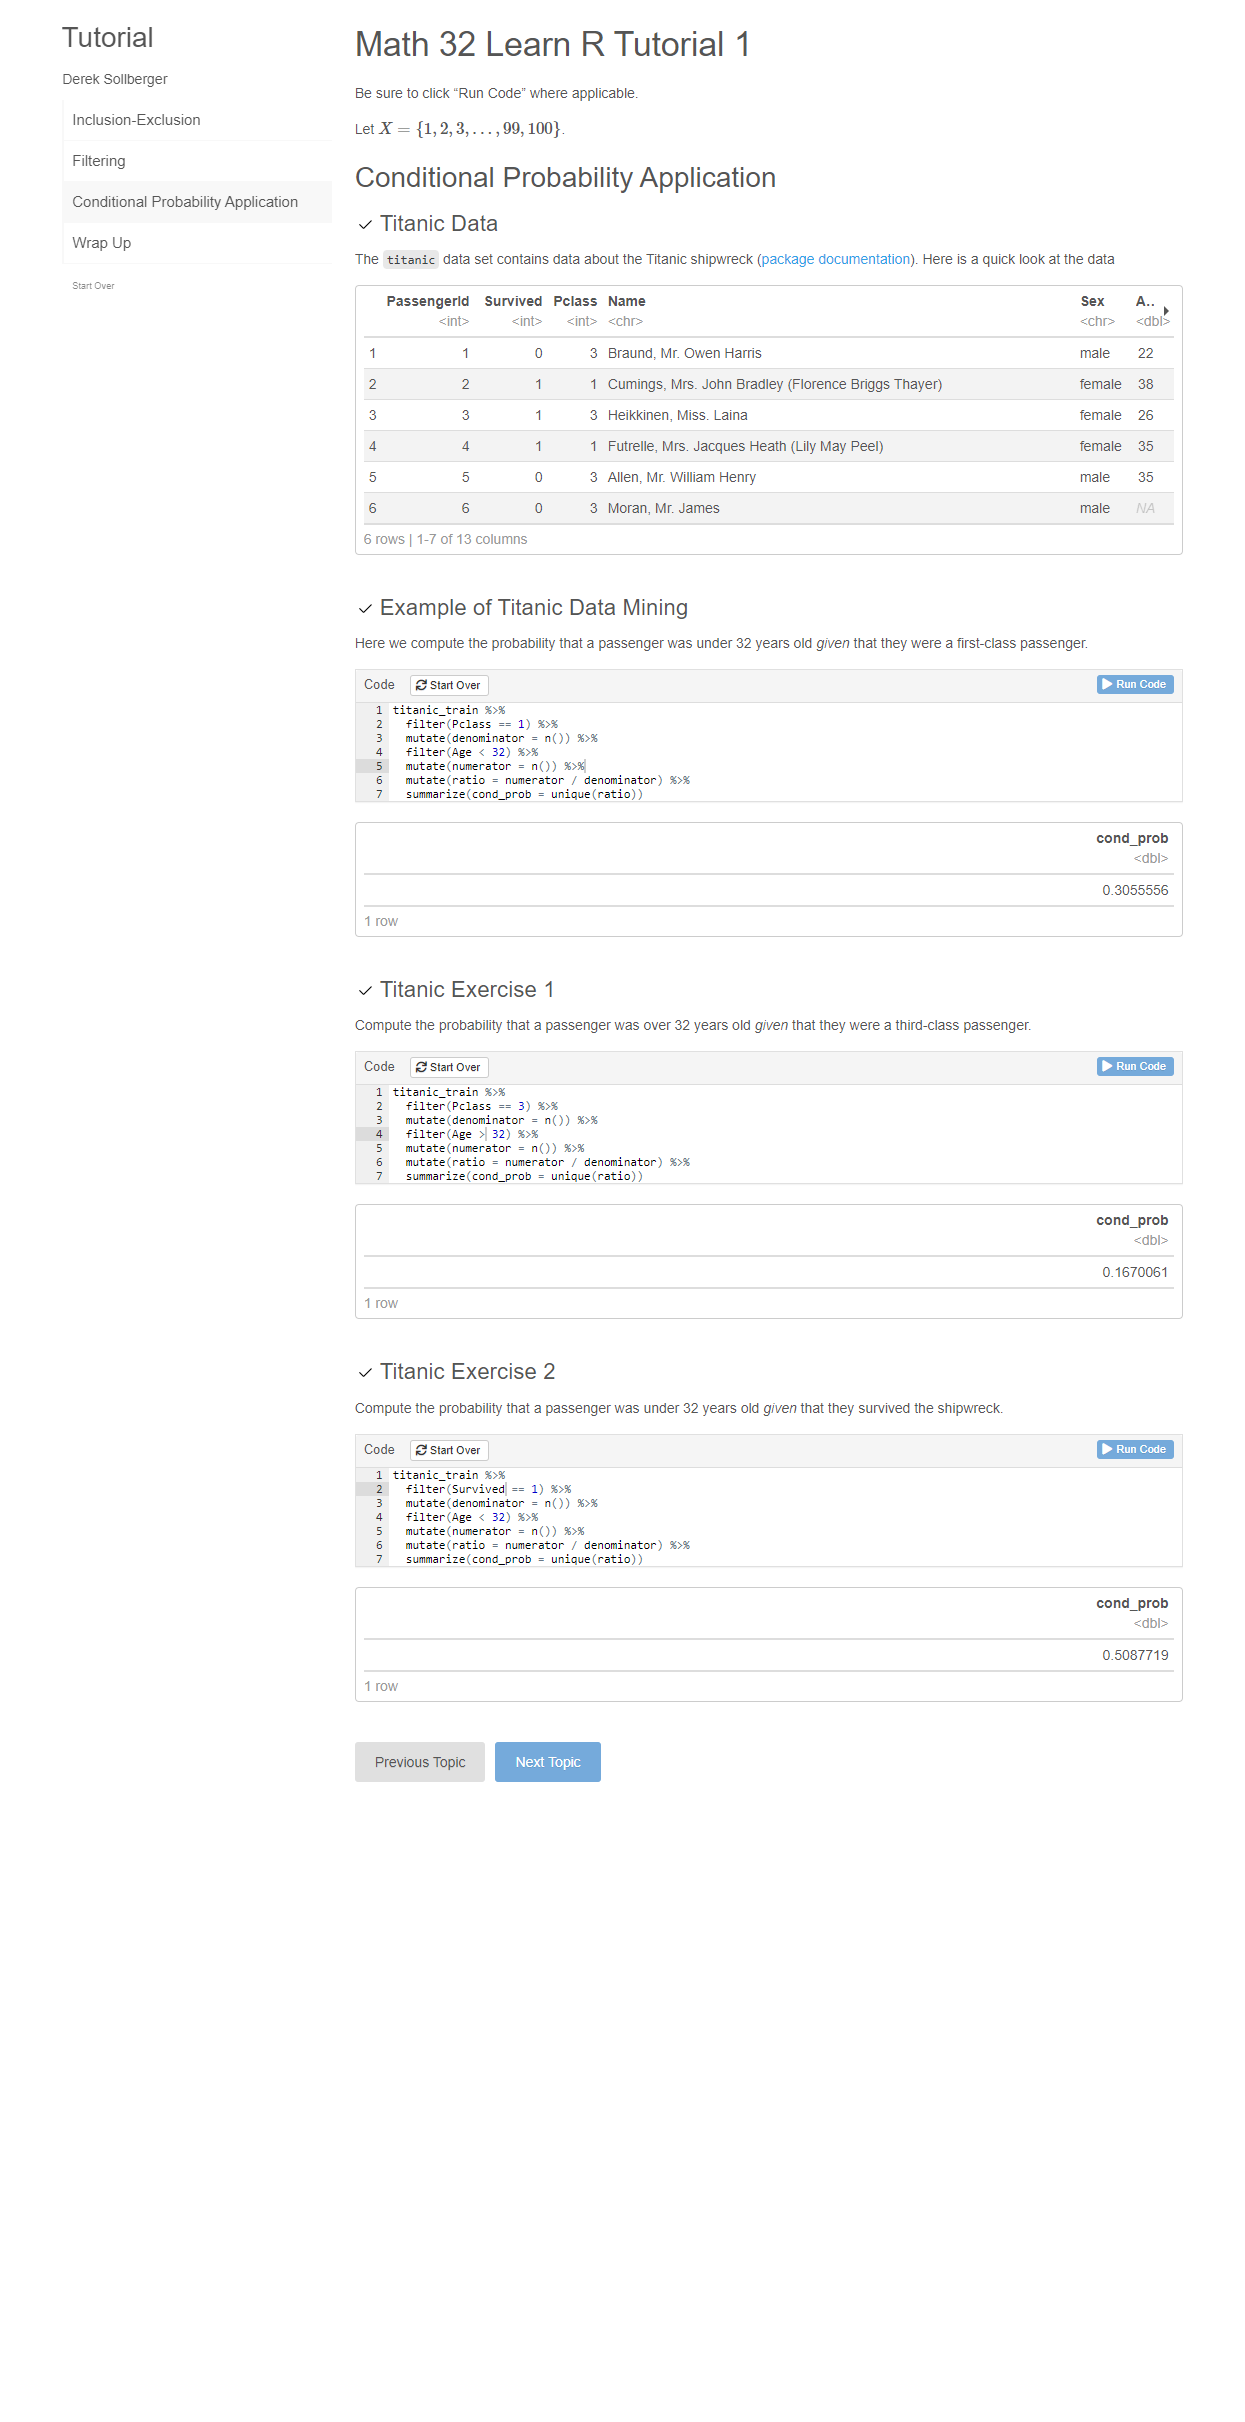
\includegraphics[scale=0.4]{page_3.png} \\
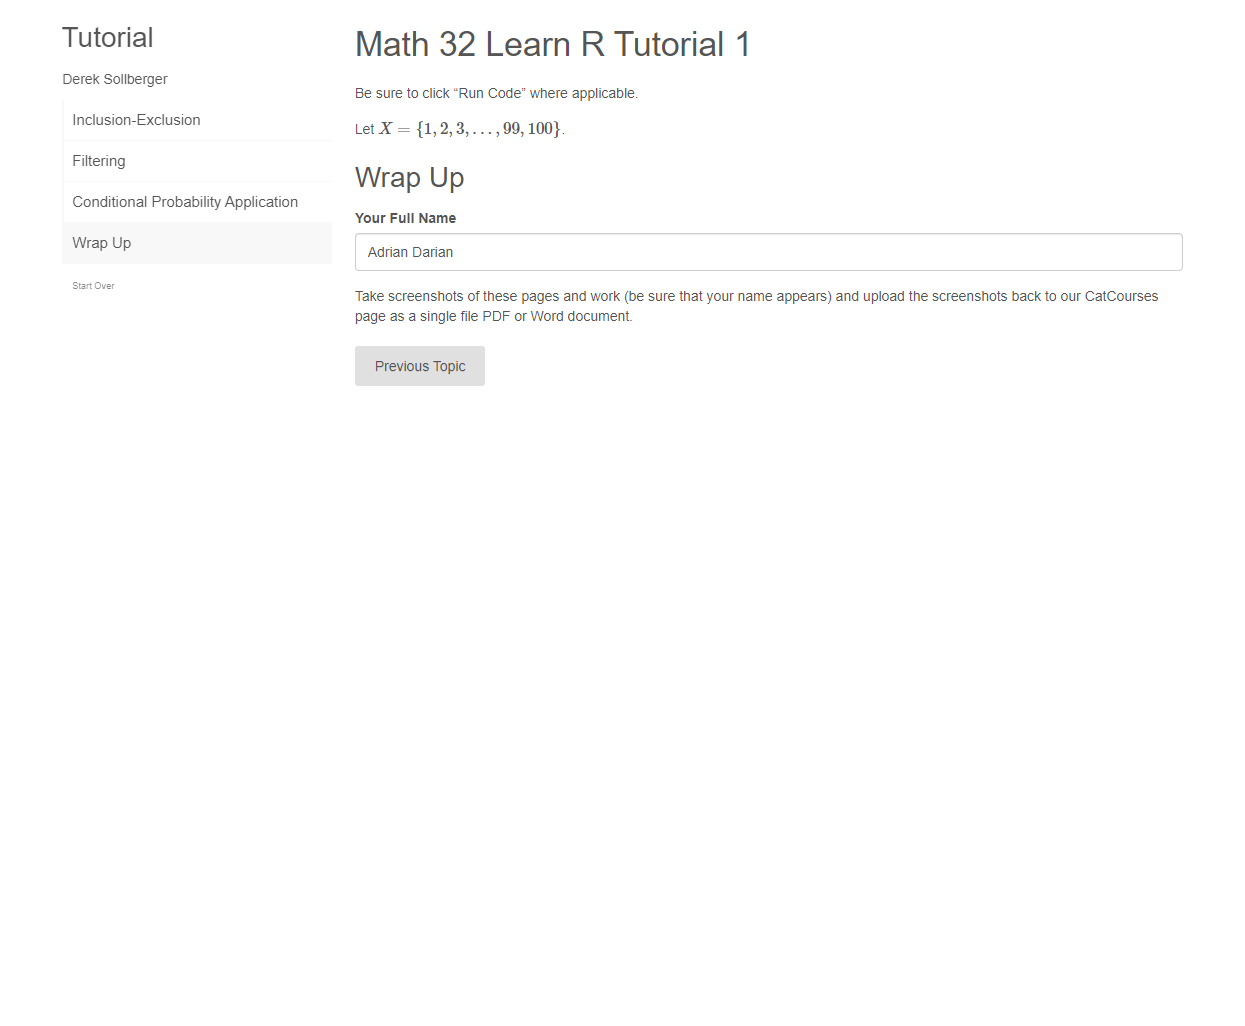
\includegraphics[scale=0.4]{page_4.png} \\
    
\end{document}